% This file was created with tikzplotlib v0.9.17.
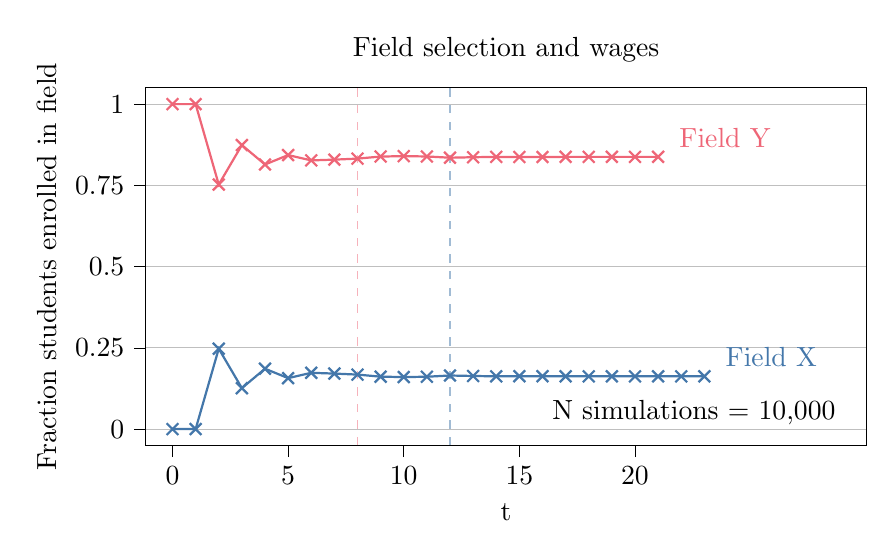
\begin{tikzpicture}

\definecolor{color0}{rgb}{0.266666666666667,0.466666666666667,0.666666666666667}
\definecolor{color1}{rgb}{0.933333333333333,0.4,0.466666666666667}

\begin{axis}[
height=6.121302808757603cm,
tick align=outside,
tick pos=left,
title={Field selection and wages },
unbounded coords=jump,
width=10.729849cm,
x grid style={white!69.0196078431373!black},
xlabel={t},
xmin=-1.15, xmax=30,
xtick style={color=black},
xtick={0,5,10,15,20},
xticklabels={
  \(\displaystyle 0\),
  \(\displaystyle 5\),
  \(\displaystyle 10\),
  \(\displaystyle 15\),
  \(\displaystyle 20\)
},
ylabel={Fraction students enrolled in field},
ymajorgrids,
ymin=-0.05, ymax=1.05,
ytick style={color=black},
ytick={0,0.25,0.5,0.75,1},
yticklabels={
  \(\displaystyle 0\),
  \(\displaystyle 0.25\),
  \(\displaystyle 0.5\),
  \(\displaystyle 0.75\),
  \(\displaystyle 1\)
}
]
\addplot [thick, color0, mark=x, mark size=3, mark options={solid}]
table {%
0 0
1 0
2 0.2474
3 0.126
4 0.1858
5 0.1568
6 0.1732
7 0.1708
8 0.1677
9 0.1613
10 0.1601
11 0.1611
12 0.1649
13 0.1634
14 0.1624
15 0.1628
16 0.1627
17 0.1623
18 0.1623
19 0.1623
20 0.1623
21 0.1623
22 0.1623
23 0.1623
};
\addplot [thick, color1, mark=x, mark size=3, mark options={solid}]
table {%
0 1
1 1
2 0.7526
3 0.874
4 0.8142
5 0.8432
6 0.8268
7 0.8292
8 0.8323
9 0.8387
10 0.8399
11 0.8389
12 0.8351
13 0.8366
14 0.8376
15 0.8372
16 0.8373
17 0.8377
18 0.8377
19 0.8377
20 0.8377
21 0.8377
22 nan
23 nan
};
\addplot [semithick, color0, opacity=0.5, dashed]
table {%
12 -0.05
12 1.05
};
\addplot [semithick, color1, opacity=0.5, dashed]
table {%
8 -0.05
8 1.05
};
\draw (axis cs:23.5,0.1923) node[
  anchor=base west,
  text=color0,
  rotate=0.0
]{Field X};
\draw (axis cs:21.5,0.8677) node[
  anchor=base west,
  text=color1,
  rotate=0.0
]{Field Y};
\draw (axis cs:16,0.03) node[
  anchor=base west,
  text=black,
  rotate=0.0
]{N simulations = 10,000};
\end{axis}

\end{tikzpicture}
